\documentclass{article}
\usepackage{amsmath}
\usepackage[utf8]{inputenc}
\usepackage{float}
\usepackage{epsfig,graphicx}
\usepackage{xcolor,import}
\usepackage[german]{babel}
\usepackage{textcomp}
\usepackage{mathtools}

\begin{document}
\thispagestyle{empty}
			\begin{center}
			\Large{Fakultät für Physik}\\
			\end{center}
\begin{verbatim}


\end{verbatim}
							%Eintrag des Wintersemesters
			\begin{center}
			\textbf{\LARGE WINTERSEMESTER 2014/15}
			\end{center}
\begin{verbatim}


\end{verbatim}
			\begin{center}
			\textbf{\LARGE{Physikalisches Praktikum 1}}
			\end{center}
\begin{verbatim}




\end{verbatim}

			\begin{center}
			\textbf{\LARGE{PROTOKOLL}}
			\end{center}
			
\begin{verbatim}





\end{verbatim}

			\begin{flushleft}
			\textbf{\Large{Experiment (Nr., Titel):}}\\
							%Experiment Nr. und Titel statt den Punkten eintragen
			\LARGE{2. Grundgrößen der Mechanik}	
			\end{flushleft}

\begin{verbatim}

\end{verbatim}	
							%Eintragen des Abgabedatums, oder des Erstelldatums des Protokolls
			\begin{flushleft}
			\textbf{\Large{Datum:}} \Large{24.10.2014}
			\end{flushleft}
			
\begin{verbatim}
\end{verbatim}
							%Namen der Protokollschreiber
		\begin{flushleft}
			\textbf{\Large{Namen:}} \Large{Veronika Bachleitner, Erik Grafendorfer}
			\end{flushleft}

\begin{verbatim}


\end{verbatim}
							%Kurstag und Gruppennummer, zb. Fr/5
			\begin{flushleft}
			\textbf{\Large{Kurstag/Gruppe:}} \Large{Fr/1}
			\end{flushleft}

\begin{verbatim}






\end{verbatim}
							%Name des Betreuers, das Praktikum betreute.
			\begin{flushleft}
			\LARGE{\textbf{Betreuer:}}	\Large{SETMAN}	
			\end{flushleft}

\section{Dichte von Flüssigkeiten}
\subsection{Aufgabenstellung}
Wir bestimmen die Dichte einer Probeflüssigkeit mit verschiedenen Instrumenten.  


\subsection{Grundlagen und Methoden}
Dichte $\rho$: [$\rho$]=kg$m^{-3}$\\
Masse m: [m]=kg\\
Volumen V: [V]=$m^3$\\
\\
\begin{equation}
\rho = \frac{m}{V}
\end{equation}

\subsubsection*{Pyknometer:}
In ein Pyknometer kann man Flüssigkeiten mit einem sehr genau definierten Volumen einfüllen.\\
Das mit Probeflüssigkeit gefüllte Pyknometer wiegt man und zieht davon die Masse des leeren Pyknometers ab. Wird dasselbe mit destilliertem Wasser wiederholt, kann man aus der relativen Dichte die Dichte der Probeflüssigkeit bestimmen: \\

\begin{equation}
d=\frac{\rho_{probe}}{\rho_{dest}}=\frac{m_2 - m_0}{m_1 - m_0}
\end{equation}

wobei die Dichte des destillierten Wassers der Tabelle im Anleitungstext entnommen wird. 

\subsubsection*{Waage:}
Die Dichte der Probeflüssigkeit wird mithilfe des Archimedischen Prinzips bestimmt: \\
Auf einen in ein Fluid eingetauchten Körper wirkt eine Auftriebskraft, die betragsmäßig mit dem Gewicht des vom Körper verdrängten Fluids übereinstimmt. \textit{aus Wagner, Reischl, Steiner: Einführung in die Physik}

\subsubsection*{Digitales Densitometer:}
Das Densitometer gibt im Gegensatz zu den vorigen Messgeräten die Dichte direkt an. Sie muss also nicht erst berechnet werden.\\
Allerdings ist darauf zu achten, dien Kolben zuerst einmal auszuspülen und erst beim zweiten Einspritzen die Messung durchzuführen.

% ______________________________________Teil 1: Ergebnisse_____________________________________________
\subsection{Durchführung}
Wir dachten, dass wir genau und ohne Ausreisser gemessen hatten - erst im Nachhinein fiel uns auf, dass wir einen Fehler gemacht haben mussten. Wir haben mit dem Pyknometer darauf geachtet, dass möglichst genau gleich viel von jeder Flüßigkeit im Pyknometer war, als wir sie wogen, indem wir überständige Flüßigkeit mit sehr saugfähigem und weichem Papier, auf dem auch eine Katze abgebildet war, absaugten. 
\subsection{Ergebnisse}

\textbf{Messung mit Pyknometer}
\begin{center}
\begin{itemize}

$m_0$=25.318g \hspace{1cm} Masse des leeren Pyknometers bei 23.2°C \\
$m_1$=77.501g \hspace{1cm} Masse des Pyknometers mit destilliertem Wasser \\
$m_2$=79.507g \hspace{1cm} Masse des Pyknometers mit Probeflüssigkeit \\
\end{itemize}
\end{center}
Die Dichte von destilliertem Wasser bei 23.2°C wurde der Tabelle im Anleitungstext entnommen: $\rho_{dest}$=997.4887$\frac{g}{dm^3}$=0.9975$\frac{g}{cm^3}$
\begin{gather*}
d=\frac{\rho_{probe}}{\rho_{dest}}=\frac{m_2 - m_0}{m_1 - m_0}\\
\rho_{probe}=\rho_{dest}\cdot\frac{m_2 - m_0}{m_1 - m_0}= \\
= \rho_{dest}\cdot\frac{m_o}{m_u}= 0.9975\cdot\frac{79.507 - 25.318}{77.501 - 25.318} \\
\Delta \rho_{probe}=\sqrt{(\frac{\delta\rho}{\delta m_o})^2\Delta m_o^2+(\frac{\delta\rho}{\delta m_u})^2\Delta m_u^2} \\
\Delta m_o = \Delta m_u = \Delta m_1 + \Delta m_0 = \Delta m_2 + \Delta m_0 = 0.002g \\
\Delta \rho_{probe}=\pm6\cdot10^{-5}\frac{g}{cm^3} \\
\rho_{probe}=(1.035846  \pm 0.00006 )\frac{g}{cm^3}
\end{gather*}
\textbf{Messung mit Waage}
\begin{center}
\begin{itemize}

$m_{Luft}$=30.021g\hspace{1cm}Gewicht des Senkkörpers in Luft\\
$m_{Fluid}$=-10.285g \hspace{0.7cm}Gewicht des Senkkörpers in der Flüssigkeit\\
\end{itemize}
\end{center}
Das Gewicht des Senkkörpers in der Flüßigkeit wurde ermittelt, nachdem wir das Gewicht des in der Luft an der Waage hängenden Körper als neues Nullniveau tariert hatten. Also entspricht das gemessene negative Gewicht dem Auftrieb, der durch die Flüßigkeit verursacht wird. Nach dem archimedischen Prinzip ist das das Gewicht der verdrängten Flüßigkeit. \\ 
 \\
Wir ermitteln die Korrektur für den Auftrieb des Senkkörpers in der Luft, indem wir die Masse m(a) der Luft berechnen, die dem Volumen V des Senkkörpers von 10c$m^3$entspricht:
\begin{equation}
m(a)=\rho(a) \cdot V=1.2\frac{kg}{m^3}10\cdot10^{-6}m^3=1.2\cdot 10^{-5}kg=1.2\cdot  10^{-2}g
\end{equation}
Nachdem unsere Waage auf $10^{-3}$g genau misst, ist die Korrektur von 1.2 $10^{-2}$g notwendig. Wir erhalten damit
\begin{equation}
m_{Fluid korr}=m_{Fluid}+m(a)=10.285g+1.2\cdot  10^{-2}g=(10.297 \pm 0.002)g 
\end{equation} 
Der Senkkörper hat ein Volumen V von 10c$m^3$. Damit ist die Dichte der verdrängten Flüßigkeit:
\begin{equation}
\rho_{probe}=\frac{m_{Fluid korr}}{V}=(1.0297 \pm 0.002) \frac{g}{cm^3}
\end{equation}
\textbf{Messung mit digitalem Densitometer}
\begin{gather*}
\rho=(0.9773 \pm 0.0001 )g/cm^3 \\
T=23^{\circ}C
\end{gather*}
Für die Messungen mit der Waage Sartorius LC verwendeten wir ihre Messunsicherheit von 0.001g, was ihrer letzten darstellbaren Stelle entspricht, und für die Mit dem Densitometer die Unsicherheit des Geräts mit seiner letzten Stelle von 0.0001g. \\
Wir verwendeten bei allen Berechnungen die in der Aufgabenstellung angegebenen Werte für die Dichte von Luft und Wasser.

% ______________________________________Teil 1: Diskussion_____________________________________________

\subsection{Diskussion}
\textbf{Vergleich der Messergebnisse}
\begin{gather}
\text{Mit dem Pyknometer:}\hspace{0.3cm} \rho=(1.035846  \pm 0.00006 )\frac{g}{cm^3}\\
\text{Mit der Waage:}\hspace{0.3cm} \rho=(1.0297 \pm 0.002) \frac{g}{cm^3} \\
\text{Mit dem Densitometer:}\hspace{0.3cm} \rho=(0.9773 \pm 0.0001 )\frac{g}{cm^3}
\end{gather}
Wir bemerken unterschiedliche Ergebnisse, die nicht in ihren jeweiligen Vertrauensbereichen liegen, vor allem fällt uns der stark abweichende Wert vom Densitometer auf. Wir könnten nun denken, dass, nachdem das Densitometer doch das genaueste Messgerät ist, dieser Wert der bessere sein sollte. Aber uns fällt auf, dass die am Densitometer gemessene Dichte \textbf{unter} der Dichte von Wasser bei dieser Temperatur liegt, wobei wir am Beginn klar gemessen haben, dass ein gewisses Volumen der Probeflüßigkeit \textbf{schwerer} als das gleiche Volumen Wasser ist, also muss ihre Dichte \textbf{höher} als die von Wasser sein. Wir haben wohl mit dem Gerät schlecht gemessen oder das Gerät hatte eine Fehlfunktion und es fiel uns leider nicht rechtzeitig auf. \\
Dass die Ergebnisse der beiden anderen Messungen nicht in ihre Unsicherheitsbereiche fallen, erklären wir durch unsere Ungeschicktheit bei einem der vielen Arbeitsschritte- Flüßigkeiten werden herumgeschüttet, Dinge aneinander gehängt, insgesamt viele Dinge bewegt - wahrscheinlich waren wir irgendwann ungeschickt. \\
\textbf{Dichte von Festkörpern}
Man könnte die Dichte von Festkörpern natürlich einfach mit dem archimedischen Prinzip messen: Man wiegt den Festkörper und ein randvolles Glas von Flüßigkeit. Dann misst man die Dichte der Flüßigkeit mit dem Densitometer. Man gibt den Festkörper jetzt in die Flüßigkeit, wobei Flüßigkeit ausrinnt. Dann wiegt man die Flüßigkeit nochmal - dabei ist so viel Volumen ausgeronnen wie auch der Körper hat. Aus der Dichte der Flüßigkeit und der Masse des ausgeronnen Volumens kann man sich das Volumen berechnen - also hat man jetzt die Masse und das Volumen des Festkörpers, deren Quotient seine Dichte ist! Heureka!
% ______________________________________Teil 2_____________________________________________
\newpage
\section{Experimente am Luftkissentisch}

\subsection{Aufgabenstellung}
Wir analysieren nun kinematische und dynamische Zusammenhänge. 
Im Anfang eine gleichmäßig beschleunigte Bewegung; dann eine kräftefreie Bewegung mit Rotationsanteil; schließlich einen elastischen, sowie einen inelastischen Stoß zweier Gleiter unterschiedlicher Massen. Wir wollen dabei lernen mit einfachen mechanischen Größen und der Beschreibung mit Vektoren umzugehen. 

\subsection{Grundlagen und Methoden}

Auf einem Luftkissentisch lassen sich Gleitkörper, die auf einem Luftkissen sitzen, nahezu reibungsfrei bewegen. Diese zeichnen Striche auf ein darunterliegendes Papier, mithilfe derer ihre Bewegung im Nachhinein analysiert werden kann. 


% ______________________________________Teil 2: Ergebnisse_____________________________________________

\subsection{Ergebnisse für die gleichmäßig beschleunigte Bewegung}
 Wir befestigen eine Masse von $m_g$=50.0g über eine Rolle an einem der Gleiter und lassen sie über den Tischrand hängen, so dass sie von der Schwerkraft beschleunigt wird und eine annähernd gleichmäßige Beschleunigung auf den Gleiter ausübt.

\textbf{Bewegungsgleichungen}
Die Bewegungsgleichung ist die altbekannte Gleichung für die gleichmäßig beschleunigte Bewegung:
\begin{equation}
\vec{x}(t)=\vec{x_0}+\vec{v_0}t+\frac{1}{2}\vec{a}t^2
\end{equation} 
mit $\vec{x_0}$ = 0 und $\vec{v_0}$=0.
\begin{figure}[H]
\caption{Bewegungsdiagramm}
\begin{center}
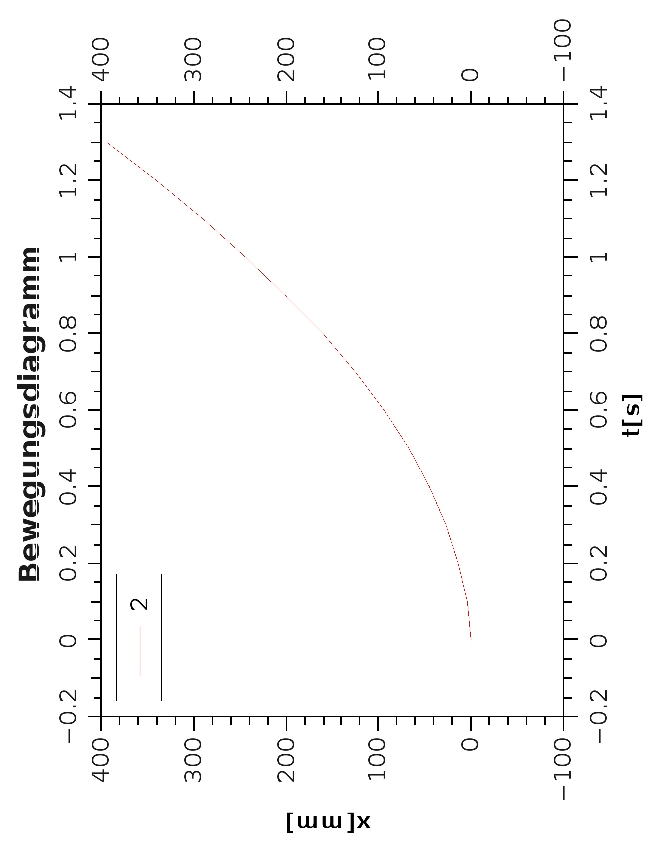
\includegraphics[scale=0.7,angle=-90]{glmbeschlBewegDiag.eps}
\end{center}
\end{figure}

\begin{figure}[H]
\caption{Geschwindigkeit}
\begin{center}
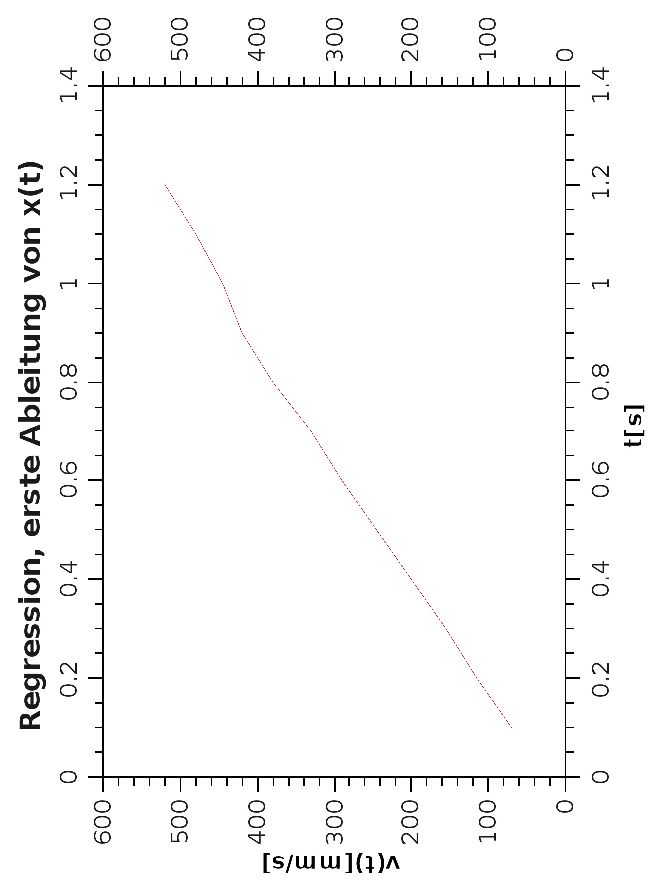
\includegraphics[scale=0.7,angle=-90]{RegressionGeschw.eps}
\end{center}
\end{figure}
\begin{figure}[H]
\caption{Beschleunigung}
\begin{center}
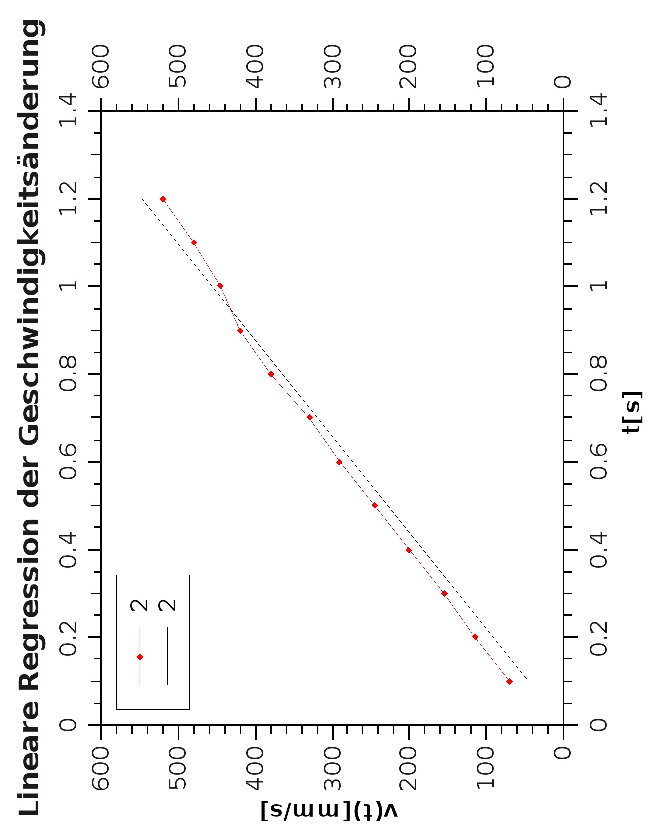
\includegraphics[scale=0.7,angle=-90]{GlmBeschlRegrBeschl.eps}
\end{center}
\end{figure}

Die Beschleunigung $\vec{a}$ erhalten wir mittels linearer Regression mit qtiplot aus der ersten Ableitung des Bewegungsdiagramms, also dem Geschwindigkeitsdiagramm: \\

Steigung der an der ersten Ableitung der Ortsfunktion gefitteten Gerade (also die Beschleunigung:) \\
A (slope) $\pm$ Err = 455.84 $\pm$ 7.6

\textbf{Kraft und Gleitreibungskoeffizient}
\begin{gather*}
a=A\pm Err=2\cdot 455.84 \pm 7.60=(455.84\pm 7.60)\frac{mm}{s^2}= \\
=(460\pm8)\frac{mm}{s^2}=(0.46\pm0.008)\frac{m}{s^2}
\end{gather*}
Aus dieser Beschleunigung, die der Gleiter erfuhr, können wir uns jetzt über die bekannte Masse $m_1$=50.0g des Senkgewichts und die Erdbeschleunigung die scheinbare Masse $m_G$ berechnen, die der Gleiter besitzt. Scheinbar deswegen, weil in ihr noch die Gleitreibungskraft enthalten ist, die der Beschleunigung entgegenwirkte.
\begin{gather}
F=m_1*a_g=m_G*a=50.0g*9.81\frac{m}{s^2}=m_G*0.46\frac{m}{s^2} \\
m_G=\frac{50.0g*9.81\frac{m}{s^2}}{0.46\frac{m}{s^2}} \\
m_G=1078.0g
\end{gather}
Mit Gaußschem Fehlerfortpflanzungsgesetz:
\begin{equation}
m_G=(1078.0 \pm18.5)g
\end{equation}
Weil wir vergessen haben ihn zu wiegen nehmen wir an, der Gleiter habe die Masse m=1000g (verschiedene Leute glauben, er habe ungefähr diese Masse.) Dann ist der Quotient aus der scheinbaren Masse, die er durch die Gleitreibung besitzt, und seiner schweren Masse der Gleitreibungskoeffizient $\mu_G$:
\begin{equation}
\frac{m_G}{m}=1.078\pm0.0185
\end{equation}


\subsection{Ergebnisse für die kräftefreie Bewegung}

\textbf{Schwerpunktgeschwindigkeit}

\textbf{Winkelgeschwindigkeit}

\textbf{Peripherie-Geschwindigkeitsvektor}


\subsection{Ergebnisse für den elastischen Stoß}

Wir beschweren Gleiter 1 mit einem Gewicht von $\Delta$m=54.6g und führen die Stoßbewegung aus. Die beiden Gleiter bewegen sich gegeneinander und leicht dezentral, mit annähernd konstanten Geschwindigkeiten. \\

\textbf{Geschwindigkeitsvektoren}
Wir bezeichnen alle Vektoren vor dem Stoß mit x, alle Vektoren nach dem Stoß mit x'.
\begin{gather}
|\vec{v_1}|=0.390 \pm 0.0005 \frac{m}{s} \hspace{0.4cm}
|\vec{v_1'}|=0.475 \pm 0.0005 \frac{m}{s}
\\
|\vec{v_2}|=0.378 \pm 0.0005 \frac{m}{s} \hspace{0.4cm}
|\vec{v_2'}|=3.19 \pm 0.0005 \frac{m}{s}
\end{gather}
\textbf{Impulsvektoren}
Wir bezeichnen die Masse eines Gleiters (wir nehmen an, dass beide Gleiter die gleiche Masse haben) mit $m_G$. \\
Durch Einzeichnung eines Koordinatensystems und Abtragung der Komponenten der Geschwindigkeitsvektoren auf dieses konnten wir folgende Vektoren ermitteln:
\begin{gather*}
\vec{p_1}=m_G+\Delta M
\begin{pmatrix*}[r]
3.9 \\ 0
\end{pmatrix*} \hspace{0.4cm}
, \vec{p_2}= 
m_G\begin{pmatrix*}[r]
-1.8 \\ 3.3
\end{pmatrix*}\hspace{0.4cm}
\vec{p_1'}=
m_G+\Delta M\begin{pmatrix*}[r]
-0.5 \\ 4.8
\end{pmatrix*}\hspace{0.4cm}
\vec{p_2'}=m_G\begin{pmatrix*}[r]
2.8 \\ -1.6
\end{pmatrix*} 
\end{gather*}

\textbf{Überprüfung des Impulssatzes}
Wenn wir $\vec{p_1}$ und $\vec{p_2}$ sowie $\vec{p_1'}$ und $\vec{p_2'}$ addieren, erhalten wir:
\begin{equation}\label{impuls1}
\vec{p_1}+\vec{p_2}=(2m_G+\Delta M )\begin{pmatrix}
2.1 \\ 3.3 
\end{pmatrix} 
\end{equation}
\begin{equation}\label{impuls2}
\vec{p_1'} + \vec{p_2'} =(2m_G +\Delta M )\begin{pmatrix}
2.3 \\
3.2
\end{pmatrix} 
\end{equation}

Aus dem Vergleich von \ref{impuls1} und \ref{impuls2} erahnen wir, dass der Impuls im elastischen Stoß nahezu erhalten geblieben ist. Die Beträge der beiden Vektoren ähneln sich noch mehr als die Vektoren selbst (3.91 und 3.94), also gehen wir davon aus, dass ihre Abweichung voneinander hauptsächlich durch die Ungenauigkeit unserer Messung und durch die Ungenauigkeit unserer Auswertung, die aus Arbeit mit Geodreieck, Bleistift und müden Augen besteht, entsteht. Allerdings ist der Stoß natürlich nicht perfekt elastisch, es ist etwas Bewegungsenergie durch die Verformung der Federn und durch die Gleitreibung verloren gegangen. \\
\textbf{Kinetische Energie}\\
Die Energieerhaltung für den elastischen Stoß besagt, dass die kinetische Energie vor dem Stoß und nach dem Stoß die gleiche ist:
\begin{equation}
\frac{Mv^2}{2} \text{vor Stoß} = \frac{Mv^2}{2}  \text{nach Stoß} 
\end{equation}
Der Betrag der Geschwindigkeit des Schwerpunkts hat sich von vor dem Stoß: 0.391m/s zu 0.394m/s nach dem Stoß verändert. Es ist natürlich nicht zu erwarten, dass die Geschwindigkeit zugenommen hat. Aber wenn wir uns mit dem Gaußschen Fehlerfortpflanzungsgesetz die Unsicherheiten der Beträge der Geschwindigkeiten anschauen, kommen wir der Wahrheit schon ein Stückchen näher, sie ergibt sich nämlich zu 
\begin{equation}
\Delta v=\pm 0.001 \frac{m}{s}
\end{equation}
Für diese Unsicherheiten haben wir allerdings nur die Unsicherheit in unseren Längenmessungen verwendet, die Unsicherheit in der Zeit, die durch die Maschine und durch die Auftragung auf dem Papier gegeben ist, wurde noch nicht berücksichtigt. Auf jeden Fall liegen zusammen mit der menschlichen Unsicherheit die beiden Vertrauensbereiche der Geschwindigkeiten, zu denen die kinetischen Energien direkt proportional sind (die Massen haben sich sicher nicht messbar geändert), schön nahe beieinander:
\begin{gather*}
v_{vorher}=(0.391 \pm 0.001) \frac{m}{s} \\
v_{nachher}=( 0.394 \pm 0.001) \frac{m}{s}
\end{gather*}
\textbf{Schwerpunkt}


\subsection{Ergebnisse für den inelastischen Stoß}
Wir beschweren Gleiter 1 mit einem Gewicht von $\Delta$m=54.6g und führen die Stoßbewegung aus.
\textbf{Geschwindigkeitsvektoren}

\textbf{Impulsvektoren}

\textbf{Überprüfung des Impulssatzes}

\textbf{Schwerpunkt}

\textbf{Kinetische Energie}


% ______________________________________Teil 2: Diskussion_____________________________________________


\subsection{Diskussion}
\textbf{Gleichmäßig beschleunigte Bewegung: Ermittelte und theoretisch wirkende Kraft}


\textbf{Kräftefreie Bewegung: }


\textbf{Elastischer Stoß: Diskussion der kinetischen Energie}

\textbf{Elastischer Stoß: Diskussion der Bahnkurve des Schwerpunktes}


\textbf{Inelastischer Stoß: Diskussion der Bahnkurve des Schwerpunktes}

\textbf{Inelastischer Stoß: Kinetische Energie}

\end{document}
